\chapter{校外实习指南}
\begin{introduction}
\item 套瓷流程
\item 暑期研学
\item 毕业设计
\item 签证办理流程
\item 经验贴
\end{introduction}

极高的研学交流以及深造比例一直是科大引以为傲的亮点。飞跃手册中传承了多少代学长的经验，荫泽多少后代。

交流实习是飞跃申请的预演，初次接触和办理这样一个复杂的流程，不仅仅是对个人信息收集能力的考验，也是个人心态的一场考试。相信经历过后会大有收获。


\section{交流学习是什么？}

\sout{交换学习按照时间可以分为短期交换、学期交换、学年交换；按照目的可以……}

交换学习种类非常之多，按照目的基本可以分为课程交换、研究实习、游学访问类三种。
课程交换类可以分为暑期、寒假课程以及学期（课程）交换，其主要的目的是前往所属学校进行对应学期课程交换，食宿以及课程费用自付。
%询问邢定一
研究实习类则主要包括暑期实习以及毕业设计，科大学生申请最多。
%询问叶祉淩；陈思琦

例如25年加州欧文分校的暑期课程交换：

\begin{presentbox}
    \begin{itemize}
        \item 项目内容：课程以培养学生大学基础科研技能为重点，让学生可以根据自己的需求选择2周，4周，及6周的课程，在课程时间不冲突的情况下，学生还可以选1-3个的课程主题。多个开学期日以及时间安排灵活性，能让课堂更多元化，清晰的先修课程要求指引能确保学生选到最适合自身水平的课程。此外，学生将有机会在UCI学习期间参加大学里举行的各种演讲、参观、会议和社交活动，与其他本地美国在校学生进行互动，培养实用科研技能，获得宝贵的美国名校经验，为进入竞争激烈的大学科研或开始职业生涯做好准备。课程的评分标准将按A-F字母等级进行评分，课程结束后，学生将会获得UCI正式的成绩单和结业证书。

        \item *项目费用包括不可退还的200美元申请费、学生服务费、每学期两门课程的学费以及每周的客座讲座/演示。
        
        *2周语言与交流课程的费用还包括每周四小时的对话伙伴时间。
        
        2-Week Session: \$1,395
        
        4-Week Session: \$2,590
        
        6-Week Session: \$3,785
        
        8-Week Session: \$4,680

        *可选费用：
        
        -2-Week UCI Dormitory Stay (2-Week Summer Academic Session only): \$2,000*
        
        -4-Week UCI Dormitory Stay (4-Week Summer Academic Session only): \$3,700*
        
        -UCI Health Insurance: \$75 per week
        
        -Airport Pick-Up Service: \$75 one way (LAX to UCI)
        
        -Weekend culture activities: price varies

        *住宿为双人间，包含三餐；
        *入选本项目的本科生可参与USTC Fellowship本科生国际交流项目资助评审。

        \item 硬性要求：外语要求：托福60及以上或同等水平，能够接受全英文授课；成绩要求：建议GPA3.0以上（不需要提供成绩单）；年龄要求：年满18岁的大学生。
    \end{itemize}
\end{presentbox}

例如25年麦马项目，该项目每年都比较热，大家可以重点关注一下：
%问沈睿阳；杨丰源

\begin{presentbox}
    \begin{itemize}
        \item 为推进与我校的战略国际合作关系，麦克马斯特大学从2019年起，面向我校本科生执行暑期研究实习项目。经与麦克马斯特大学国际处协商，2025年暑期研究实习项目的导师课题采用开放式申请模式，学生可进入官网（https://www.mcmaster.ca/），在各学院教职工介绍部分（如工程学院：https://www.eng.mcmaster.ca/about/faculty）选择2-3名意向导师，申请加入其项目参与相关课题研究。
        
        \item 硬性要求：年级要求：我校全日制正式注册大二或大三本科生；专业要求： 与麦克马斯特大学目标导师研究实习要求一致；学业要求： 基础扎实、成绩优良，无不及格成绩。语言要求： 托福≥80/雅思≥6.5。

        \item 项目费用免项目费。国际旅费、食宿费、护照签证费等其他个人消费自理
    \end{itemize}
\end{presentbox}

例如25年UGVR项目，该项目与Stanford合作，清北以及中科大三所学校共同选拔学生，不同学院每年名额约为2-3，会变化浮动，竞争激烈。

\begin{presentbox}
    \begin{itemize}
        \item 申请流程：
        登陆“全球化学习化平台” 网址：http://vista.ustc.edu.cn/ 点击项目列表-GVP项目-“2025年夏季学期斯坦福大学SoE UGVR本科生暑期研究实习项目”进行申请，在”项目文件“上传申请材料，请选择2-3名教授作为备选导师，一名备选导师需要上传一份申请材料。请学院相关负责老师在申请截止3个工作日内前登录系统完成相关审核与推荐工作。

3.申请材料及提交要求如下：

申请材料：

（1）英文简历(Resume)

（2）英文个人陈述及申报理由（Statement of Purpose）

（3）英文成绩单（教务处开具的正式英文成绩单,official transcript）

（4）1-3封英文推荐信（如推荐老师直接将推荐信发送给拟申报教授，请上传相关证明）

（5）英语能力证明（大学英语四、六级、雅思、托福等）

（6）其他能证明科研能力的材料，视个人情况自行决定是否提交

相关要求：

（1）所有申请材料提供原件扫描版即可，请将申请材料（1）-（6）扫描并按顺序合成一份PDF文件；

（2）如有申请材料是中文的，请自行提供英文翻译,一并附在相应PDF文件中；

（3）PDF命名格式：项目序号 - 拟选导师姓名- 申请者姓名拼音 (如 1-Anton Ermakov - LU Juanjuan)。（项目序号见附件）

注意事项：

（1）此项目注重科研能力，有接收教授直接审核材料，请务必在个人简历中着重个人在申报领域的科研经历。

（2）往届录取学生申请材料见附件，供参考，请勿外传，谢谢！

(3) 暂未办理护照的申请者，请尽快办理。

        \item 硬性要求：年级要求：2022级（大三）正式注册全日制本科生;专业要求：学科知识扎实，研究经历突出;学业要求：GPA≥3.5;语言要求：TOEFL≥89 (如暂无托福成绩，申请阶段可暂不提交。如被录取，学生最迟需2025年2月初之前提交托福成绩单)

        \item 特别提示：斯坦福大学特别提示，请申请者不要在申请阶段与斯坦福课题教授直接联系。
    \end{itemize}
\end{presentbox}

通过上述范例大家应该已经清楚这几种交流学习有什么区别了。

\section{暑研基本流程以及重要时间节点}

本书的重点放在了研究实习。


\begin{itemize}
    \item 12月前：准备简历（CV）；准备一个模板化的个人陈述（PS）方便后续使用；transcript（教务处可导出）；推荐信可以不必准备。
    \item 12月-次年3月：套瓷
    \item 4月-7月：手续办理
    \item 7月开始：项目开始
\end{itemize}
\begin{remark}
    \begin{itemize}
        \item 研究实习既可以私套，也可以套瓷一些公开招聘信息。私套自由度大、范围广，导师方向可能更契合；公开招聘范围受限，但往往有往届师兄去过，一则可提前打听，二则有口碑保障。值得一提的是，很多招聘信息是往届学长在飞跃群中发布的，今年甚至有人不知道飞跃群里有招聘贴。
        
        \item 私套可以直接发给大老板，也可以发给 postdoctoral fellow（博士后）。其实大老板邮箱常由手下 Ph.D 或 post fellow 代看，真正带你做项目的，往往也是 post fellow。
        
        \item 招聘信息时间不固定，一般 12 月左右会出现第一批。建议在此之前准备好 CV，便于及时套瓷。暑研本质上是先到先得。若遇到心仪的招聘信息，一定尽快投递。若 4 月后仍未套瓷成功，也无需气馁，飞跃群也有同学 5 月成功套到项目。 
        
        \item 由于近期情况有变，签证问题也是需要考虑的重要因素，。签证常规流程一般会经历1-2个月的时候。到达美国适应生活可能还需要一周，如果套瓷太晚，可能拿不到推荐信。
        
        \item 套瓷的目标是申请研究实习，包括暑研和毕设，可任选其一或同时申请。邮件务必写清类型。暑研通常为两个月，毕设一般六个月。为了降低培训成本，有些导师更倾向招收毕设学生。北大学生因大四还有必修课，研学时间短，在短期项目（如 UGVR）上有优势；长时间暑研则科大学生可能更占优势。
        
        \item 暑研套瓷比 Ph.D 申请更需注意套瓷道德。若导师明确表示接收意愿，请勿轻易拒绝，否则可能给未来 Ph.D 申请留下不良印象。
        
        \item 语言成绩是否必要？理论上办理流程中不要求。如果面试交流无障碍，一般无需语言成绩。但官方项目（如 UGVR）可能会要求 TOEFL 90 分以上等硬性条件。
    \end{itemize}
\end{remark}

具体的套瓷以及导师查询就放在套瓷篇了。

\notetitle{套瓷}
\section{套瓷}
\begin{notebox}[写在前面]

套瓷的过程可能充满了惊喜（可能更多的是失望）。

公知乾卦九四否？“或跃在渊，无咎”：新事物带着时代势不可挡的锐气与旧事物决斗，但由于历史惯性，旧事物仍然强大。此时，新旧事物的对决就好像人面对着深渊往对岸跳——可能掉入深渊；可能成功抵达。因为可能落入深渊就不去跳么？假使真的掉入深渊呢？卦象告诉我们：“无咎”——没有关系，大胆去做吧！

\end{notebox}

套瓷时需要选择导师，导师选择是一个非常重要的环节。导师的选择直接影响到你在实验室的科研方向、研究内容、工作氛围等。导师选择部分请参看第~\ref{sec:导师选择}~章节内容。

\subsection*{套瓷以及注意事项}

找到心仪的导师后，就可以写套瓷信进行套瓷，正式的套瓷一般要发送一封CV、cover letter、PS(Propose of Statement)。

\subsection{CV}
CV主要是用来介绍自己的教育背景、科研经历、技能等。CV应该简洁明了，突出自己的优势和与实验室研究方向的匹配度。一般来说，CV应该包含以下几个部分:
\begin{itemize}
    \item 个人信息：姓名、联系方式、学校、专业等
    \item 教育背景：学校、专业、学位、GPA等
    \item 科研经历：实验室名称、研究方向、工作内容等
    \item 技能：编程语言、实验技能等
    \item 其他：获奖情况、实习经历等
\end{itemize}

出国申请Ph.D.以及国内申请夏令营的CV要求略有不同，二者不宜等同。本文着重介绍出国申请Ph.D.的CV要求。夏令营的CV要求可以参考小红书等经验贴。

UGVR提供往年学长学姐们的CV以作参考，可以登录\href{https://vista.ustc.edu.cn/}{Visa.ustc}-国际GVP项目，找到往期的UGVR项目，会附带各种材料，包含推荐信、PS，非常全面。一般按照其格式修改即可。CV书写力求简洁明了。

\subsection{Cover letter}
\textbf{Cover letter}是求职信的意思，主要是用来介绍自己以及表达对该实验室的兴趣。一般来说，cover letter应该简洁明了，突出自己的优势和与实验室研究方向的匹配度。
对于cover letter的建议，来源于飞跃群，作为参考。

\begin{presentbox}
大概是不要写太多废话和比较空的东西（

比如要写出跟这个教授的针对性，而不是全篇闭着眼介绍自己

讲具体对教授的什么研究感兴趣，自己的技能如何match或者能参与正在进行的项目

以及再明确在位置讲明白自己写邮件干什么（什么时候多长时间，什么资金来源，intern还是phd），这些关键的不要让对方回复邮件再问一遍（

招收一个国外的intern要走那么多流程老复杂了 也要花精力时间去指导，呆的时间还不长，“来了能很快上手干活”或者“来了之后对我的实验进度有帮助”是比较重要的，至少会要求个人过去已经有了相关的很基础的知识储备，加上一点点本领域的研究经历，来了才能很快参与进来。总不能期望没有什么match背景的来待4个月 其中一半2个月在教很基础的东西慢慢培训上手

至少背景相似 过去的科研经历可以支撑自己interview的时候聊个十几分钟（

但这个match我觉得不用限制特别小的方向，比如说原来做离子阱平台量子计算的可以去找冷原子的量子模拟，甚至固态体系NV center 甚至超导的量子计算，甚至偏EE相关的比如integrated optics，量光器件 只要有点沾边都可以去尝试联系，当然越相近，对未来PhD申请也会更好

\hfill ——发自诗佳姐姐的手机
\end{presentbox}

某学长的套瓷信如下：

\begin{presentbox}

\noindent Dear Professor XXX，

\noindent My name is *, a junior student majoring in life science at Division of Life sciences and Medicine, University of Science and Technology of China. I gained xxx/4.30 GPA and ranked top *in our department. I got * , *, and * respectively in the courses “*”, “*” and “*”, which offers me solid theoretical back-ground. In addition, I have joined * lab in my university for over a year and did some ** works.

\noindent I am fascinated by your research in ** and it is a perfect match with my desired research direction. Since I am fully self-financed, may I ask whether there is any in-ternship opportunity in your lab around summer 2023? My resume is in the attachment.

\noindent Looking forward to hearing from you soon.

\noindent Best regards,

***
\end{presentbox}

泛泛的好处是消耗精力少，对面导师浏览的速度快；但是坏处就是太过泛泛，难以吸引对面导师的兴趣。

笔者主要采取了飞跃群群友的建议。

\begin{presentbox}
\noindent Dear Prof. *,\\[0.5ex]

\noindent This is Enchong Zhao, a junior in Bioscience at University of Science and Technology of China (USTC). I am writing to apply for \textbf{any undergraduate internship position} in your laboratory for the 2025-2026 academic year. I am excited about your research in biochemistry and epigenemics. I am longing for the opportunity to learn from your team’s groundbreaking research.\\[0.5ex]

\noindent \textbf{Regarding my education}, my current GPA is 3.73/4.3. USTC places emphasis on foundational courses in mathematics and physics, and these courses help me understand the biological process. I got 92 and 90 respectively in the courses of "Cell BiologyⅠ" and "Bioinformatics".\\[0.5ex]

\noindent \textbf{Concerning my research experience}, in my first year, I \textbf{joined the USTC iGEM team} and my contribution included transforming, cultivating, and fermenting the yeast, which gave me practical experience with microbial culture and molecular biology techniques. Building on this, in my second year, I \textbf{joined Prof. Song Xiaoyuan’s laboratory}, which focuses on the transcriptional role of 3D genome and long non-coding RNAs (lncRNAs) in brain aging. I led a project for the 9th CULSC competition, investigating regulatory factors that maintain the topologically associating domain (TAD) using Tetrahymena thermophila as the model system. Since it has unique and defined TAD boundary sequences, it allowed us to use CRISPR-dCas9 system to capture the TAD boundary binding protein. I gained valuable experience about the genomic and molecule biology, which I believe that it matches your filed about the epigenomics. Thus, I think this internship is a valuable experience for me to further deepen my knowledge about epigenemics.\\[0.5ex]

\noindent \textbf{Pertaining to my skills}, I have worked extensively with LaTeX for scientific reports, MATLAB for experimental data processing and SnapGene for plasmid construction. In the bioinformatics class, I conducted the data analysis of ChIP-seq, RNA-seq and part of the scRNA-seq using the Linux system and R, which I believe can be helpful for the internship project.\\[0.5ex]

\noindent \textbf{To conclude, my background in molecular biology, genomics and bioinformatics will ensure that I will quickly fit in your laboratory and complete the internship satisfactorily}.\\[0.5ex]

\noindent \textbf{Attached is my CV for your review}. I would be grateful for the opportunity to further discuss my application in an interview. Thank you for your consideration, and I am looking forward to hearing from you.\\[0.5ex]

\noindent Enchong 
\end{presentbox}

恰当的换行、适当的加粗，简单的细节就可以极大提高邮件的可读性。该邮件较长，考虑到教授可能不会很有兴趣打开附件类型的PS文件查看，就将cover letter和PS合在一起。附件添加CV。

仅作参考！

\begin{itemize}
    \item 发送邮件时，标题务必简洁明了，例如 \texttt{Summer Internship Application}。
    
    \item 邮件格式要规范，避免语法和拼写错误。可使用 Grammarly 等工具检查（当然也可以请 ChatGPT 润色，并提醒它补充逻辑语句以增强连贯性。但据说经过 AI 润色的信件往往“有迹可循”，慎重考虑）。
    
    \item 本示例更偏向海套风格，部分实验室（例如麦马项目）若要求学术套瓷，请务必留意相关说明。
    
    \item 注意时差！尽量设置定时发送，在对方工作日上午 9:30 左右投递（美国不像中国统一用北京时区，建议自行确认当地时区）。
    
    \item 附件务必规范，仅附 CV 或 PS，格式建议为 PDF，以免被系统退回。
    
    \begin{figure}[H]
        \centering
        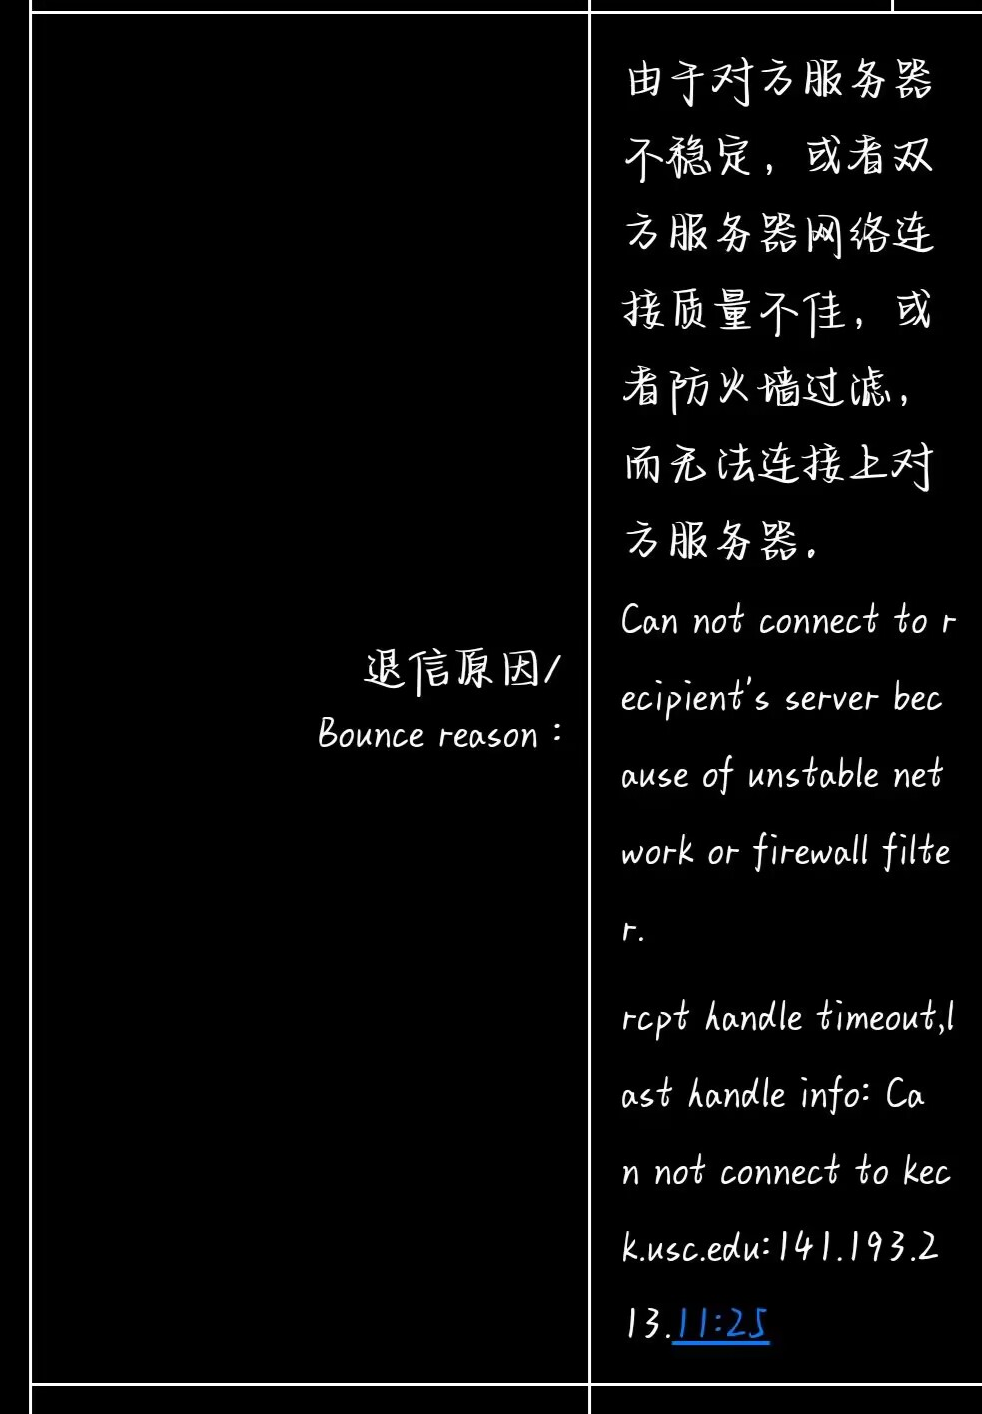
\includegraphics[width=0.24\linewidth]{image/交流学习/退信.png}
        \caption{因神秘不可抗力被退回的信件}
    \end{figure}
    
    \item 陌生邮箱可能被识别为垃圾或病毒邮件。科大邮箱一般没问题，但若有条件，建议注册谷歌邮箱以备不时之需。
    
    \item 除非十分着急，不建议同时联系同一机构的多位老师。老师们若相互交流，发现你广撒网，可能会影响印象。当然，同时联系不同机构的老师问题不大。
\end{itemize}

\begin{remark}
    如果你发现套瓷回复率极低，按完全属于正常情况，不要气馁。不回复往往是默拒或者压根没看到甚至进了垃圾桶，可以隔4-7工作日follow up一下。笔者以及身边的生院学生套瓷数量往往10+，回复率不足30\%，十分幽默。其他专业回复率高，往往大于1/3。（不知道的还以为学生物犯了天条）。此时套瓷华人导师或者实验室里面的华人博后可能会有效果。

    套瓷结果往往与成绩、科研经历等有关，也与领域、运气有关系。
\end{remark}

\section{面试}

\begin{notebox}[写在前面：]

能够看到这里，说明你很可能已经成功和老师建立了交流关系，但前路仍然漫漫，不要懈怠哦。

乾卦九三告诉我们，“君子终日乾乾，夕惕若，厉无咎”。意思就是说啊，君子整天自强不息，勤勉不懈，晚上还时刻保持警惕。现在虽然会存在着危险，但是不会造成灾难。革命尚未成功，同志尚需努力哦~ 
\end{notebox}

\IfNeededPageBreak{2.5cm} % 预留图片高度+间距

\begin{wraptable}[8]{r}{0.45\textwidth}
    \vspace*{-0.5\baselineskip}
    \centering
    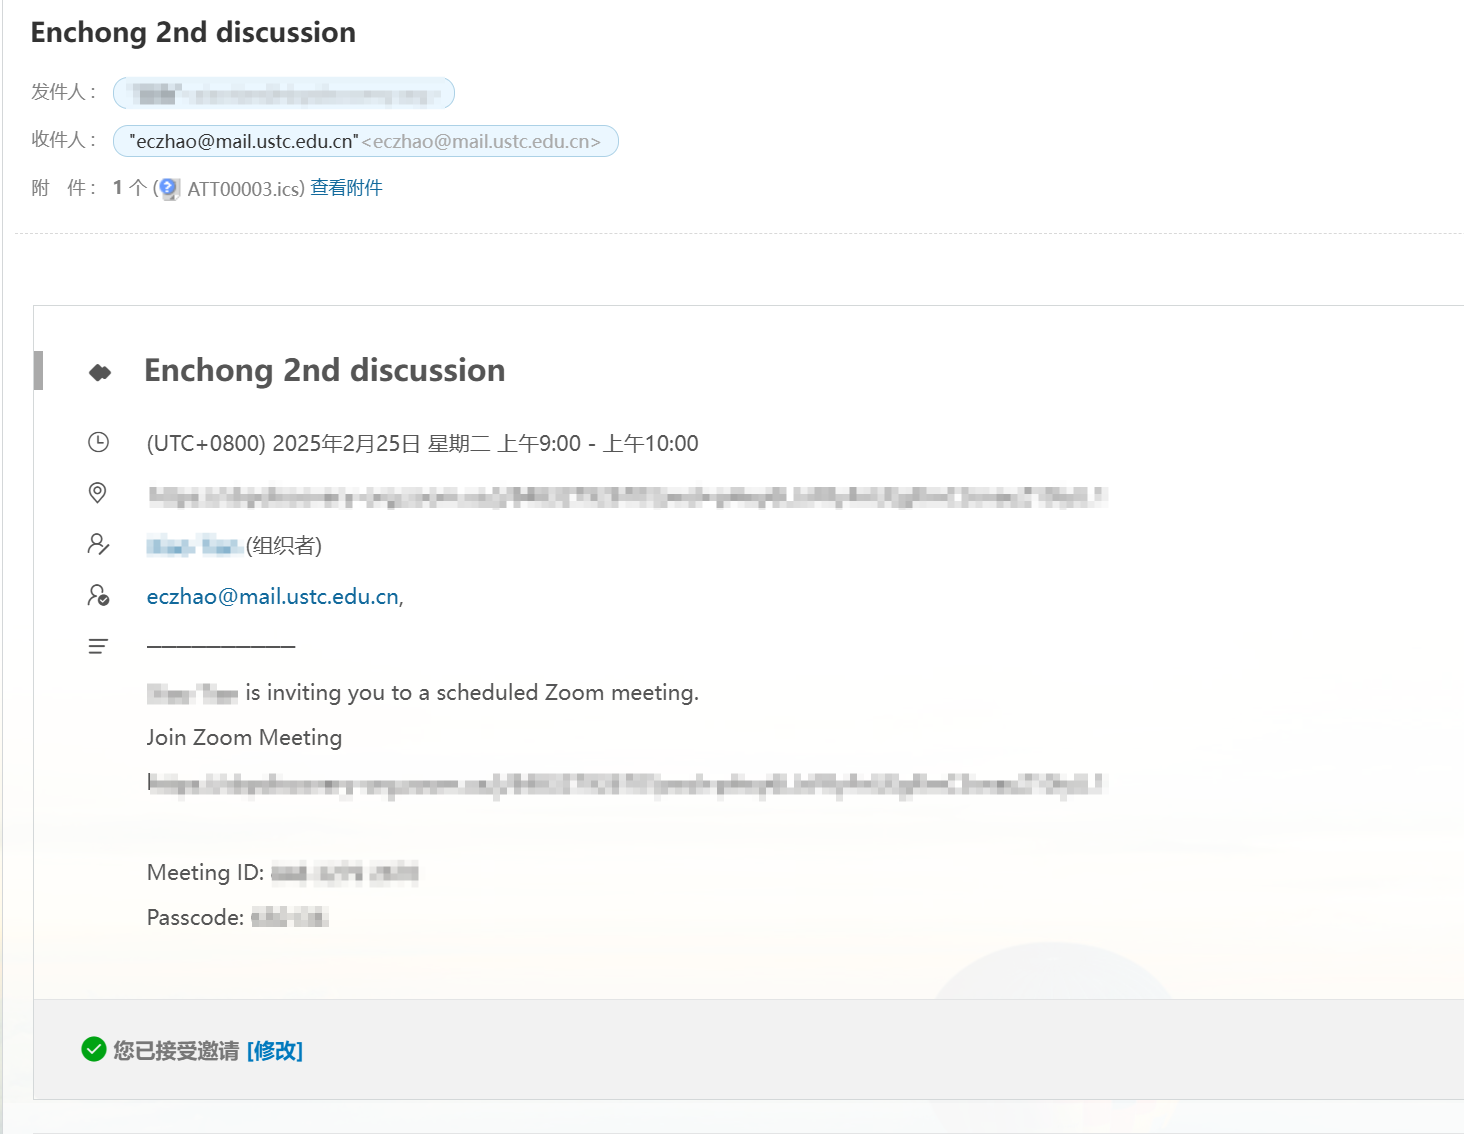
\includegraphics[width=\linewidth,height=5cm]{image/交流学习/zoom.png} % 固定高度
    \caption*{\small Zoom邮件预约界面示意图}
\end{wraptable}

常见的面试软件有 Zoom、Skype 等，有些机构可能会使用 Microsoft Teams 等软件。

Zoom workspace 软件的使用需要梯子，但是账号创建并不需要 Google 账号。建议使用发送邮件的邮箱去创建账号，预约过并同意后，对方老师往往会友好地提示你面试是 informal 的，不需要准备 slide（deck）。

当然也有老师会明确提示需要准备 PPT，如图所示为预约确认邮件。

\vskip 50pt

面试方面的内容，飞跃手册述说备矣，但是仍然要提醒：

\begin{enumerate}
    \item \textbf{面试礼仪：} 首先是着装。暑研面试一般不是非常正式的场合，不必穿正装，但务必保证干净整洁。展示个性可以，但邋遢或不精神可不是什么好个性哦。男生建议刮刮胡子，擦擦眼镜片，简单梳理头发或干脆理个发，不要让自己看起来太随意。其次是交流。说话放慢、说清楚；听不懂时礼貌请老师重复一遍；多看屏幕与老师保持“眼神交流”，必要时缩小屏幕盯着摄像头看；不要在面试中抱怨自己的学校或学长。
    
    \item \textbf{准备：} 面试前建议准备一些常见问题及自己的回答，后面我会附上上届师兄师姐提供的问题清单和我遇到的题目。最好练到脱稿也能流畅自然表达，紧张时就不至于乱说。若听力一般，可用同步翻译软件辅助，但最好还是靠自己理解回应。
    
    \item \textbf{时间问题：} 注意时差，面试常在傍晚或清晨进行。特别提醒：\lstinline{12:00 a.m.} 是零点，\lstinline{12:00 p.m.} 才是正午十二点。别问我是怎么知道的，问就是搞错过一次，很尴尬。
    
    \item \textbf{语言选择：} 面对华人导师、华人 post fellow、港澳地区老师等，无论邮件还是面试，建议先用英文，得到允许后再用中文。
    
    \item \textbf{结束后的礼貌：} 无论结果如何，都建议发封简短的感谢邮件。
    
    \item \textbf{面试轮次：} 面试通常会有两轮。第一轮了解申请者大体情况并介绍实验室；第二轮告知结果、讨论后续安排。在等第二次面试期间可以继续套瓷尝试。一旦教授明确表示愿意接收，请不要“放鸽子”。Ph.D 被鸽可能情有可原，毕竟是人生大事，但一个 intern 还这么操作就有点过分了。
\end{enumerate}

    例如： 
    
\begin{presentbox}
\noindent Hi *,

\noindent This is * from USTC. I am writing to express my sincere gratitude for the opportunity to interview with you. I truly appreciate your kind and thoughtful responses to my questions.

\noindent Wishing you a Happy Chinese New Year in advance!

\noindent Best regards,\\
\noindent Your Name
\end{presentbox}

对于华人post fellow或者华人Ph.D学生，可以发一些中国节日祝福。

对于歪果仁，也可以发一些节日祝福，例如给一位女士发邮件，恰逢3.7女生节，笔者就在结尾随意带上了一句，虽然最后也没有得到机会，但是可以感觉到会加分滴。

例如下面的回复：

\begin{presentbox} 

  \noindent   Of course.  I love that China has a Chinese Women’s Day!  I wish you a Happy Chinese Women’s Day as well!
\end{presentbox}

\begin{remark}
    如果有任何的顾虑或者打算（例如要拒绝老师），请务必真诚并且\text{礼貌}。

    例如：

    非常感谢您给予我这次宝贵的暑期实习机会，我一直非常关注并欣赏您在相关领域所做的研究工作，也非常期待能够在此次实习中有所收获。不过，由于当前美国的局势尚不明朗，签证及出入境等方面存在一定不确定性，我无法完全保证自己是否能顺利成行。与此同时，考虑到自己未来的发展方向，如若无法顺利出国，我暑期需要为申请国内的研究所或高校做准备。而目前许多国内单位的推免或考核依托于暑期夏令营，若错过报名与参与，可能会对我的后续申请造成影响。因此，在非常矛盾与不舍的心情下，我可能将不得不放弃这次赴美实习的机会，为此深感抱歉。我衷心感谢您对我的信任与支持，也希望未来还有机会向您学习。

    
\end{remark}

\textcolor{red!70!black}{\faIcon{thumbtack} }后面是一些常见问题：




\notetitle{校内申报以及签证护照}

\begin{notebox}[写在前面]

能够看到这里，说明你很可能已经拿到了offer，不可否认的是现在的快乐是真实的，但未来的烦恼也是真实的——恭喜你同时拥有两者！

拿到offer固然可喜，说明老师非常非常希望你能前往学习。但是接下来将要面临的非常重要的问题就是材料准备。

\end{notebox}

\section{材料准备}

\section*{内部申请FAQ}
{\small 请注意，该FAQ绝大多数问题得到了国合部负责人回应，少部分源自经验贴，具体请以国合部信息为准} 

\begin{qa}[资助问题]

{\small 提示：国合部网站个人中心有资助标准，请先阅读资助标准再看}

\textbf{Q1}：希望出国同时完成毕业设计以及暑期研学，请问资助时长只能是4个月吗？如果可以将资助时长延长至3（暑期研学）+4（毕业设计）月，申请有什么要注意的吗？

\textbf{A1}：可以3+4；新版国合部网站请分开申请暑研以及毕设。

\textbf{Q2}：国合部资助类型是什么？

\textbf{A2}：不国合部实行包干制，只会覆盖差旅以及生活费用；请保留相关的
\end{qa}


\begin{qa}[其他材料提交]
    \begin{itemize}
        \item 根据教务处近日发布《[2024]04号 中国科学技术大学本科生境外科研实践目管理规定(试行)》要求，学生中请境外科研实践项目须进行立项申报，过渡期间，学生须填写《境外科研实践项目开题申请表》，由校内导师签字后扫描与邀请函打包上传至全球化学习平台自主申报表单“offer文件“处。出访时间超过3个月，须请教学院长或国合院长签字审批签字。
        \item 如进行境外科研同时选课，按照已发文件要求需要同时上传任课老师知情同意书。申请境外科研实践项目时长超出三个月或者与教学学期高度重合的，原则上不能参加校内教学活动，也需要提交材料，教秘签字确认。
    \end{itemize}    
\end{qa}
\begin{qa}[资助证明办理问题]

\textbf{Q2}:资助证明如何办理？

{\small 学校开具全额的资助证明，可以省去开具bank statements的流程。但需要注意，出现任何问题，学校不予以负责！可能的问题是1.由于学校的原因，签证被拒；2.租房时无法完成资产认定，国外的租房审核往往更严格。}

\textbf{A2}:资助证明申请本身是不需要在国合部的平台上进行提交并审核的，直接开具资助证明信即可。资助证明的例文格式如下：

使用有科大抬头的纸打印，找到教秘负责人盖章即可。（注意女生要改一下'Mr.'哦，不然会很尴尬的）

需要注意，学校考虑到每一位学生的个性化选择，会给你开具资助证明，但是如果出现任何问题，需要学生自己承担。建议学生开具bank statements。一个可能的风险就是租房问题，美国的leasing office租房要求较为严格，很多不接受学校的资质证明，甚至不接受scanned或者paper bank statement，必须要美国账户的可验证的资金（流水）。具体可以看飞跃的生活篇。

\begin{remark}
    上述为国合部负责人的回应。但是实际办理时，教秘负责人会要求先完成国合部自主申请。请在邮件中说明所有情况，包括但不限于：自己的名字、学号、需要前往的学校或者研究所的名称以及地点、资质证明出现的数字是否合理（不同地区要求不同）。然后找到老师盖章。
\end{remark}

\end{qa}

\begin{figure}[H]
    \centering
    % 左边图片
    \begin{minipage}{0.48\textwidth}
      \centering
      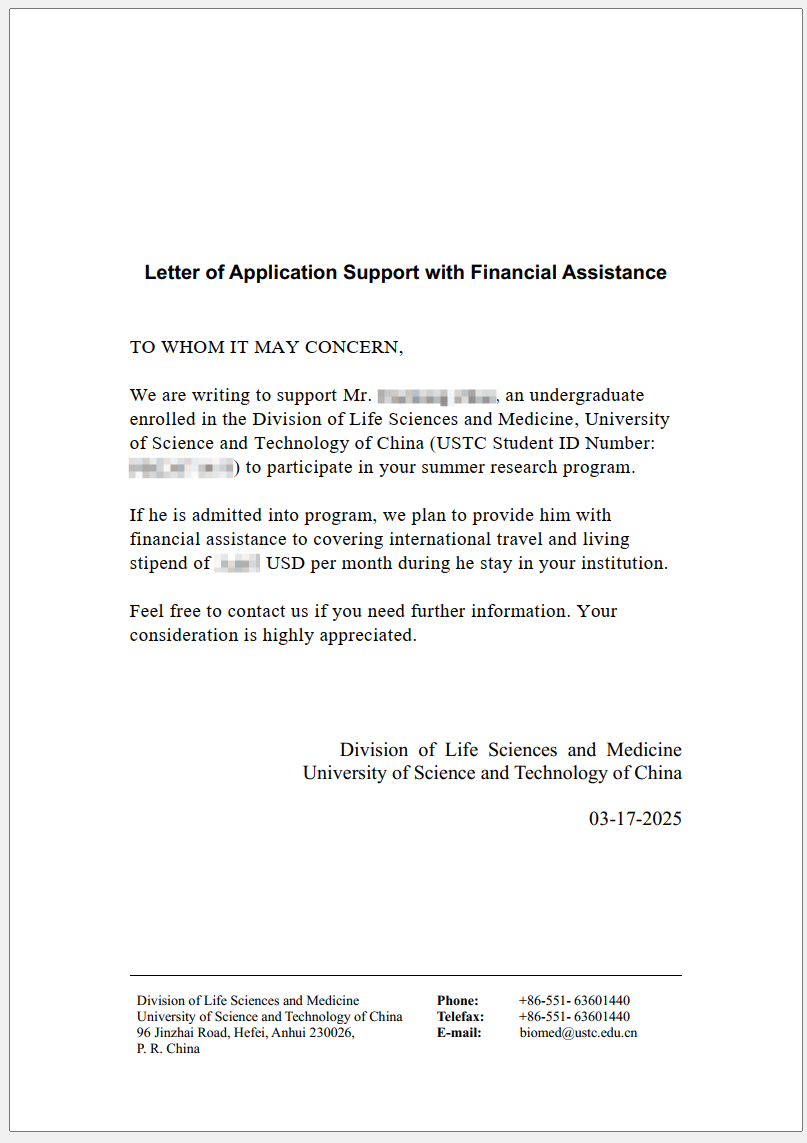
\includegraphics[width=\linewidth]{image/交流学习/资助证明.png}
        \caption{资助证明}
    \end{minipage}
    \hfill
    % 右边图片
    \begin{minipage}{0.48\textwidth}
      \centering
      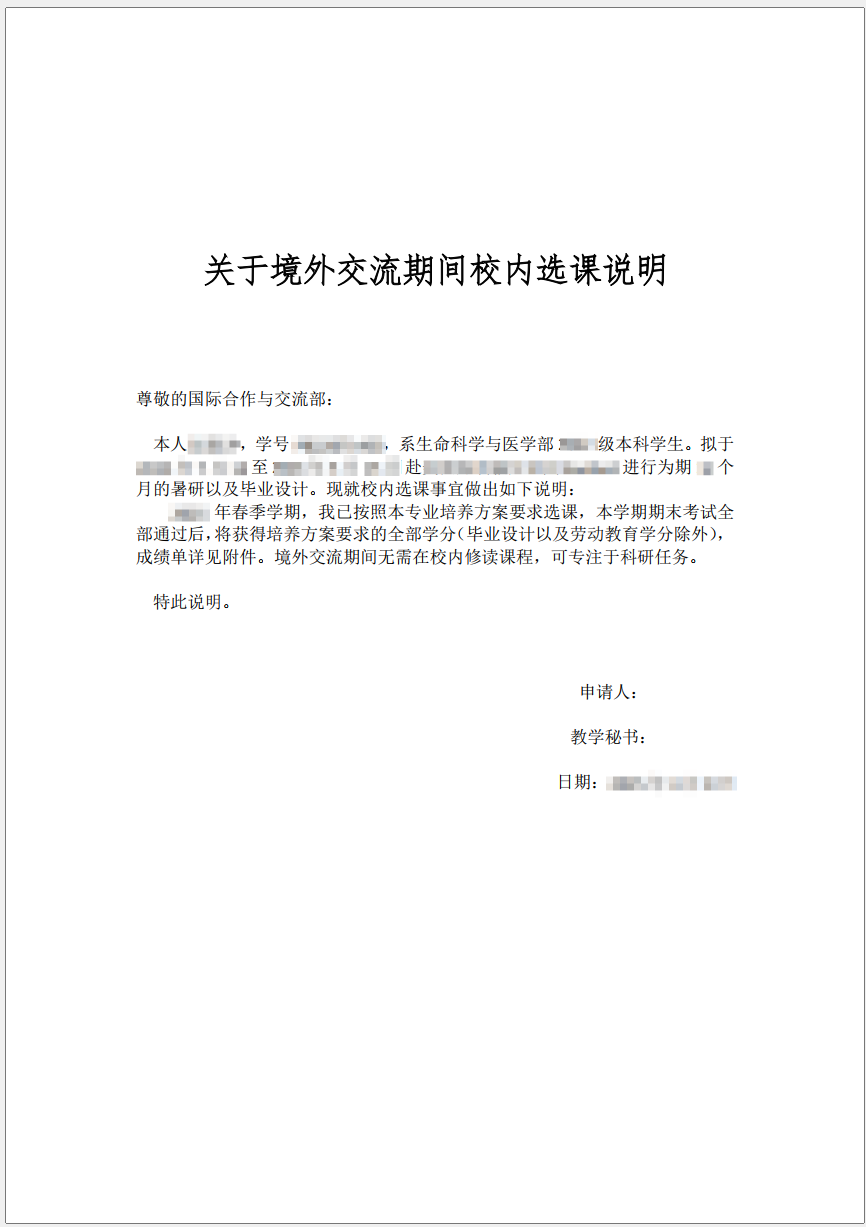
\includegraphics[width=\linewidth]{image/交流学习/境外交流期间不选课说明.png}
      \caption{境外交流期间选课说明}
    \end{minipage}
\end{figure}


\section*{暑研准备}

要注意签证sponsor不一定是实习学校，具体看签发DS-2019的是谁。如果签证的sponsor不是本校，例如CETUSA等，则签证以及保险往往由第三方机构提供，一般follow up即可。

\section*{签证护照}

\textbf{护照（Passport）}

护照由\textbf{本国政府}签发，是证明持有人国籍和身份的正式证件。

\textbf{护照的作用}
\begin{itemize}
    \item 允许持证人\textbf{出入境自己的国家}。
    \item 作为国际旅行的\textbf{身份凭证}。
\end{itemize}

\textbf{签证（Visa）}

签证由\textbf{前往国家的政府}签发，允许持有人\textbf{进入该国并停留一定时间}。

\textbf{签证的作用}
\begin{itemize}
    \item 规定持证人在该国的\textbf{停留时间和目的}（旅游、学习、工作等）。
    \item 由\textbf{目标国家的使领馆}审核签发，通常贴在护照上。
\end{itemize}

\textbf{签证的有效期与停留期}
\begin{itemize}
    \item \textbf{签证有效期（Validity）}：指持证人可以在该时间段内入境该国。
    \item \textbf{允许停留时间（Duration of Stay）}：指每次入境后，最多可以停留的时间。
\end{itemize}

\textbf{护照与签证的关系}
\begin{itemize}
    \item 签证通常是\textbf{贴在护照上的一页}，必须配合护照使用。
    \item \textbf{没有护照无法申请签证}，护照有效期不足可能影响签证申请或入境。
    \item \textbf{持有签证并不保证入境}，最终决定权在于入境国家的\textbf{海关官员}。
\end{itemize}


\subsection*{护照办理}

护照办理只需要身份证即可。该部分仅告诉你在哪里可以办理，具体的办理流程认真阅读相应说明即可。

在“支付宝”-“搜索”-“移民局”-“中国公民服务”-“预约申请”，选择比较近的合肥市政务服务中心，预约后按时去办理即可。


\subsection*{签证材料准备}

常见的签证申请材料包括如下部分：

\textbf{- Proof of education}– a letter from your university confirming your \textbf{full-time} student enrollment status

\textbf{- Proof of funds}– upload a scholarship letter and/or a bank statement balance with at least \$4,167 x the number of months on your program

\textbf{- Passport}- upload biographical page only 

 \textbf{- CV}– upload your resume 
 
-\textbf{Form DS 7002–}this will be provided to you for review and to sign later in the application process.  

\subsubsection*{说明：}

\begin{enumerate}
    \item \textbf{Proof of education} 
：一般Intern身份必须是全职学生，因此该材料是为了证明你是全职学生。

该证明可以在第三教学楼证明材料处打印；该证明也可以在“综合教务处”——“电子证明导出”——“在读证明中英文”导出电子版。注意综合教务处有导出次数限制。

某些时候申请时对面机构可能会认为该证明只能证明你的在读身份(Enrollment)，不能证明你是全职的(Full-time)，这时候可以上传成绩单(transcripts)，以证明你是全职学生。

例如如下邮件往来：

A：Additionally, I reviewed the Proof of Education document and while it does confirm your enrollment, we must also receive confirmation that you are enrolled full-time. Can you either request an updated letter that confirms this, or we can consider reviewing your transcripts in addition to the letter you have. If we can determine you took a full-time course when reviewing the transcripts then this may be sufficient.

B：Attached are my transcripts and proof of current studentship. Are they enough to proof that I am full-time student?

A：Thank you for the education documents. Yes, they will suffice. I have already uploaded them to the application portal.

\item \textbf{Proof of funds}:学校开具全额的资助证明，可以省去开具 bank statements 的流程。但需要注意，出现任何问题，学校不予以负责！（可能由于是科大开具的材料，会被check）具体的开具方式请见FAQ。

\item \textbf{Passport}:

可能会要求上传护照第一页，扫描即可。

\item \textbf{CV} 申请时肯定都写过了吧

\item  \textbf{Form DS 7002：} DS-7002 是 Training/Internship Placement Plan（培训/实习计划书），是 J-1 交流访问学者签证（特别是 Intern 和 Trainee 项目）必须提交的重要文件。主要host机构填写，自己只需要签字确认即可。

\end{enumerate}

\subsection*{面签}

对于首次办理 F 或 J 签证的学生，需要前往美国大使馆或领事馆进行面签。可选择的地点包括北京、上海（通过率相对稳定）、广州（据说存在一定的拒签“指标”）、沈阳等。以下是笔者办理 J-1 面签的材料准备和流程，部分内容感谢 yfy 学长的经验分享。

面签材料准备：

必备材料：
\begin{itemize}
    \item 护照（若有旧护照，注意确认有效期）
    \item 身份证
    \item 照片（可在学校东区照相馆拍摄，直接说明“美国签证照片”即可，工作人员很熟悉要求）
    \item 学生证 
    \item \textbf{DS-2019}
    \item \textbf{DS-7002}
    \item I-901 缴费记录（工作人员会查验）
    \item DS-160 确认页（工作人员会查验）
    \item 面谈确认页（pdf 文件名通常为：预约管理 customer self-service）
    \item 保险证明
\end{itemize}    

额外支持材料（备用）：
\begin{itemize}
    \item 个人 CV
    \item 实验室介绍
    \item 导师 CV
    \item 父母资产证明
\end{itemize}

面签流程：

\noindent day 0：提前踩点，熟悉路线（包括大门、存包处）。

\noindent day 1：

注意事项：
\begin{enumerate}
    \item 面签不允许携带电子设备，务必提前存包。签证处一般会有存包点（价格偏高），也可委托朋友代为保管。
    \item 面签处通常要求迟到超过预约时间 30 分钟后不得入场。虽然近期规定有所放宽，但仍建议提前 1 小时到达。
\end{enumerate}

以北京面签为例，面签需要经过多次安检与材料查验，可参考下图路线：

\begin{figure}[H]
    \centering
    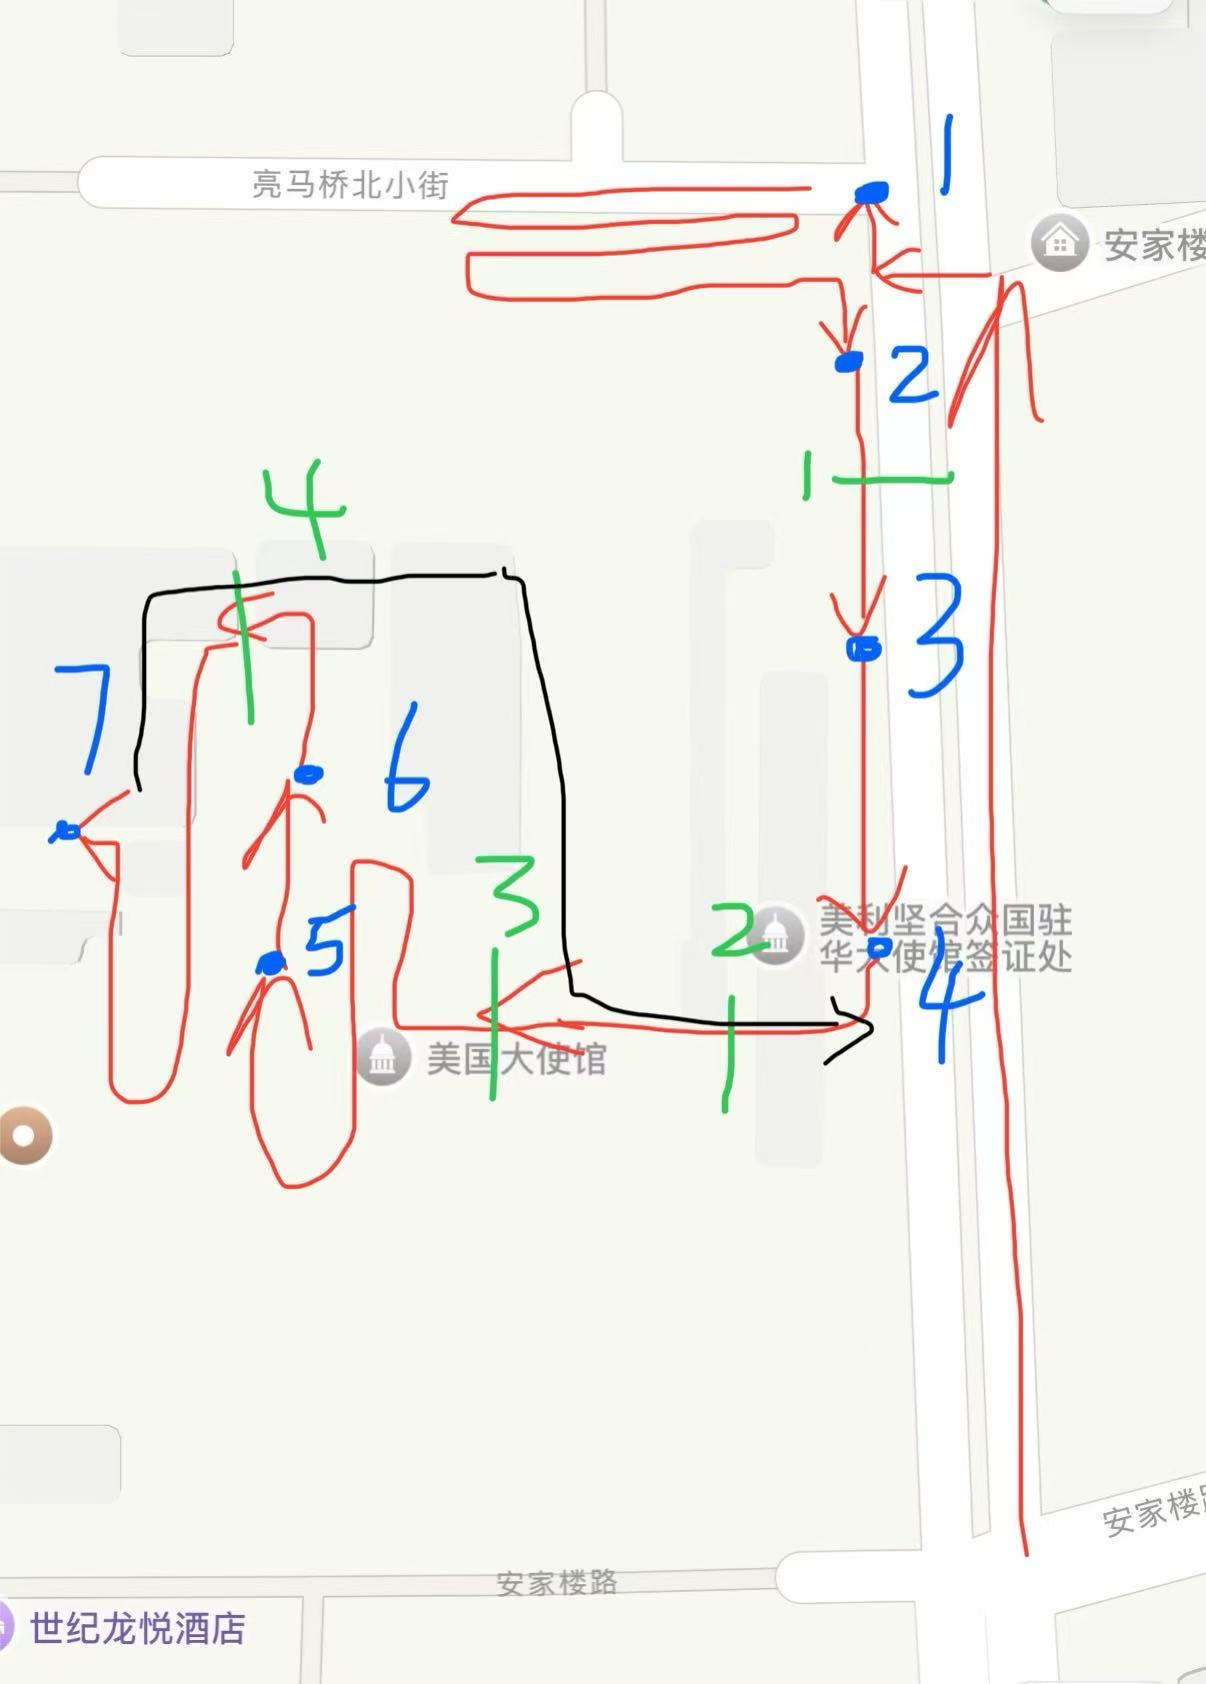
\includegraphics[width=0.6\linewidth]{image/交流学习/面签map.png}
    \caption{北京面签路径图}
\end{figure}

流程如下：
\begin{enumerate}
    \item 在亮马桥北小街排队等候，现场一般有志愿者协调入场。为保证预约时间靠前者优先入内，可能会暂时拦住后续排队人员。
    \item 第一次材料检查：武警核验身份证、DS-160 确认页和面谈确认页。建议提前将这些材料夹在护照信息页处，方便出示。
    \item 进入非移民签证通道后，工作人员再次查验护照和确认页，并在护照后贴上条形码。
    \item 通过安检（禁止携带饮品）。
    \item 穿过一段露天通道进入主楼，工作人员引导至窗口（1-7号）查验材料：需提交护照、DS-2019 和 I-901 缴费记录；可能会核对照片是否合格，如不符合要求需在馆外重拍（需现金）。随后护照会被归还。接着前往 8-13 号窗口录指纹，只需扫描护照背面条码。
    \item 完成指纹后，上楼排队等待正式面试。
\end{enumerate} 

笔者当时排队约 3 小时（早上 7 点至 11 点），但面试过程非常简短，通常几分钟即可结束。  

面签环节主要材料为 DS-2019（J签）。当时签证官特别询问了我的本科学校，我回答为 University of Science and Technology of China。面试时要特别注意，避免任何可能被解读为“非法移民倾向”的回答。例如，当被问及未来计划时，可说明“回国继续完成本科（Bachelor's Degree）”。  

\begin{figure}[H]
    \centering
    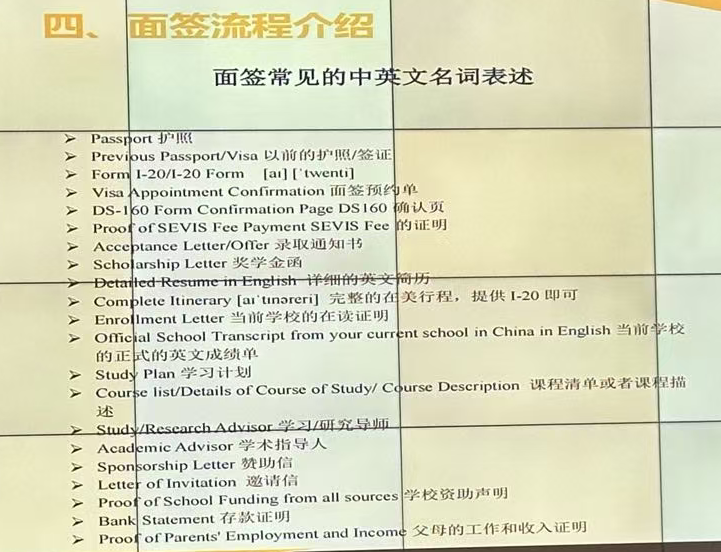
\includegraphics[width=0.5\linewidth]{image/交流学习/面签常见材料.png}
    \caption{面签常见材料及对应英文名}
\end{figure}

面试结束后，签证官会发放不同颜色的小条子，不同馆区含义可能略有差异。  

- 若顺利通过，签证官会在 DS-2019 上签名；护照被收走后，一般数日即可寄回。  

- 若进入行政审查（Administrative Processing，即“check”），通常会收到 221(g) 表格并被要求补交材料。即使如此，护照也会被收走。此时无需过度担心，按要求提交材料即可。  

补充说明：签证重新开放预约后，新增社交媒体审查。据部分同学反馈，几乎所有签证都被 check，并要求提供社交媒体账号且保持公开状态。但通常在两周内即可进入 “Approved” 状态。  
%20250825-end

\section*{保险（Insurance）}
一般来说，学校会要求购买保险，具体的保险公司和保险内容可以参考学校的要求。美国对于J-1签证的保险要求如下可以参见\href{https://j1visa.state.gov/sponsors/how-to-administer-a-program/}{BridgeUSA}。

\section*{银行卡}

如果需要提前缴费（如保险），没有SSN，可以通过国内申请外币卡或者国际电汇（International Wire Transfer）。
流程很简单，了解流程的话自己在手机上就可以完成支付。

1.支行往往办理的业务有限，不能办理visa卡。往往只有分行才能办理。

2.银行往往不会轻易给学生身份开visa卡。


%约稿沈睿阳
\section{往届招聘以及暑研lab情况}


\begin{presentbox}[2026fall]

\begin{itemize}
    \item Harvard Medical School：Professor:David Sinclair。Sinclair是著名的衰老研究专家，但是坏名声和好名声一样大。Sinclair教授的实验室主要研究衰老和衰老相关疾病的机制，尤其是与表观遗传学和代谢相关的方面。开始时间较早且很热门，The Sinclair lab非常欢迎交流生。
    但是Sinclair本人饱受争议，包括但不限于overstate相关工作（仅列举一个驳斥其核心工作的论文：Sirtuins are Not Conserved Longevity Genes）；兜售假药。感兴趣请自行Google。
    %不知道没去成算不算无形的安排？
    \item Sanford Burnham Prebys：Assistant Professor:Xiao Tian(田骁);Co-writter of "The information Theroy of Aging" with Yuancheng Lu;关键词：衰老、表观遗传、神经生物学。(24以及25年均host一名USTCer)Xiao目前还有NIA和加州的基金。
    \item MIT/Whitehead：LSRF and AFAR Postdoctoral Fellow：Yuancheng (Ryan) Lu（吕垣澄）；(24年host一名USTCer);Co-writter of "The information Theroy of Aging" with Xiao Tian;关键词：衰老、表观遗传、神经生物学。（Xiao Tian以及Yuancheng Lu曾一同在HMS"The Sinclair Lab"任博后，共同完成了综述“The information Theroy of Aging”。田老师于24年独立。二人均有多年host科大学生的经验。两个人都非常nice!）
    \item New York University;Assistant Professor:Shuo Chen(陈硕)(24年host3个USTCer；25年host1个USTCer)。人很好，申请到不少NIH基金；科大学生点击就送。由于一些原因，申请前请联系往届学长了解详情再做决断！
\end{itemize}    

\end{presentbox}

\begin{remark}
    此处提供往届暑研lab的名单，供大家参考。因为有往届学长学姐开疆拓土，大部分对USCTer印象颇好。如果对该方向感兴趣，可以尝试联系。注意，往届暑研lab的名单并不代表该实验室会继续招收暑研生，具体情况请参考各实验室的官网或者联系老师。
\end{remark}


\subsection*{其他招聘信息}

\notetitle{前言}
\begin{notebox}[写在前面]

    NIH经费被大幅缩减，25fall的Ph.D.项目offer一度缩水超过30\%，部分高校甚至出现了裁员、回收offer的情况。
\end{notebox}

笔者仅仅只完成了暑研以及毕设，未进行申请，经验有限。做任何事情之前，都建议搜小红书或者问问有经验的师兄。

%约稿沈睿阳
\section{暑研与毕设}

\subsection{行前准备}

\subsubsection*{国外消费}
一些帖子更推荐在美国办理 Visa 卡，但从实际体验来看，Visa 与 Master 并无明显区别。

借记卡中最重要的信息是卡号和卡背的安全码；到期时间、billing address 以及持卡人信息相对次要。需要特别注意的是：不要随意把卡背照片交给他人，也不要泄露卡号和安全码！

\subsubsection*{行李、电话卡与国际航班}

收拾行李前应提前了解目的地情况。在美国，大多数生活用品、食物和药品都可以方便购买。  
在准备衣物时，应结合当地气候。
电话卡方面，可以在淘宝购买临时无限流量卡用于过渡，抵达美国后再办理长期套餐。
由于宿舍以及办公场所都有WiFi，因此日常生活中也不会使用非常多的流量。

国际航班一般需提前三小时开始办理 check-in，务必留好时间。若为多段航班，托运行李要提前询问是否能直挂到最终目的地，并在中转（transfer）时确认行李去向。


\subsubsection*{租房}

\begin{itemize}
    \item \textbf{Leasing office 租房}  
    要求严格，需要可验证的资产或流水。例如加州 \textbf{Pacific Sands Apartments}：
    \begin{itemize}
        \item \textbf{费用与流程}：申请费 40 美元/人（不可退还），合租室友也需分别缴纳；申请时还需交 holding deposit（若申请失败可退还）；提交后由第三方机构（如 \texttt{twodot.com}）审核。
        \item \textbf{硬性要求}：
        \begin{itemize}
            \item 收入需达到房租的 2.5 倍（Combined gross monthly household income）。
            \item 或美国账户中有至少 7 万美元存款（必须是电子版存款证明，中国银行仅提供纸质版，不被接受）。
        \end{itemize}
        \item \textbf{申请前需确认事项}：租期（lease term）、utilities（水电垃圾费）、house insurance、是否支持信用卡支付、维修服务（maintenance）。
        \item \textbf{优惠与注意事项}：部分公寓会推出 ``首月免租'' 或 ``1000 off'' 的优惠，但务必写进合同，不要轻信口头承诺。
        \item \textbf{个人经验}：未意识到需要收入或美元存款证明，导致申请受阻；因结汇差价（约 0.003）而缺乏将大额人民币换成美元的动力。
    \end{itemize}
    
    \item \textbf{房东直租}  
    相比 leasing office，房东直租在沟通和维修上可能更麻烦，但也有一定优势：
    \begin{itemize}
        \item 租期灵活，可商议。  
        \item 流程简单，一般 “押一付一” 即可。  
        \item 审核宽松，无需复杂证明。  
        \item 部分房东倾向现金支付，以避免纳税，可与房东商议，可能获得租金优惠。  
        \item 华人房东通常更好沟通，但需谨防 ``同胞坑同胞'' 的情况。  
    \end{itemize}
    
    \item \textbf{支付与汇款}  
    若能刷信用卡，最便捷。但若不接受信用卡，通常流程是：国内账户购汇 $\rightarrow$ 转账至美国账户 $\rightarrow$ 取现支付。
    \begin{itemize}
        \item \textbf{常见方式}：
        \begin{itemize}
            \item 办理美国银行（BOA）的储蓄卡：国际汇款手续费固定约 15 美元/次，建议一次多汇。  
            \item 使用中行卓隽信用卡：每月前 5 笔 ATM 取现免手续费。  
        \end{itemize}
        \item \textbf{注意事项}：切勿直接用信用卡取现，因为会立即计息且利率极高。  
        \item \textbf{节省手续费}：如何降低成本值得研究，可以多查阅小红书等经验贴。  
    \end{itemize}
\end{itemize}


租房还要考虑是否靠近公交站便于上下班，是否方便买菜？美国的公共交通系统一般不好，公交超过30分钟时间就非常长了，毕竟一般要呆很久，每天超过1h通勤比较折磨。公交班次往往间隔30 min，能够真实体会到什么叫catch the bus。

\subsection{暑研经历}
\subsubsection*{生活与开销}

相比国内，美国的生活节奏要慢很多。刚来时，可能会觉得不适应，甚至感到焦虑或无所适从。其实这都是很正常的现象——别太紧张，take it easy，慢慢解决生活中一个个遇到的小问题就好。如果有困难，也一定要及时和导师、师兄师姐沟通请求帮助。

在日常购物中，你可能会遇到一些新的计量单位，第一次看到时难免有些迷茫。最常见的就是 lb（磅），大约0.9斤（更准确来说是 454 克）。此外，在一些袋装或单件出售的商品上，还会看到 ea（each），表示“每个多少钱”。oz，表示28 g或者28 mL。熟悉了之后，就会觉得购物也没那么复杂。

日常消费的话可以参考我帮新来的同学在VONS购物的发票：

\begin{figure}[H]
    \centering
    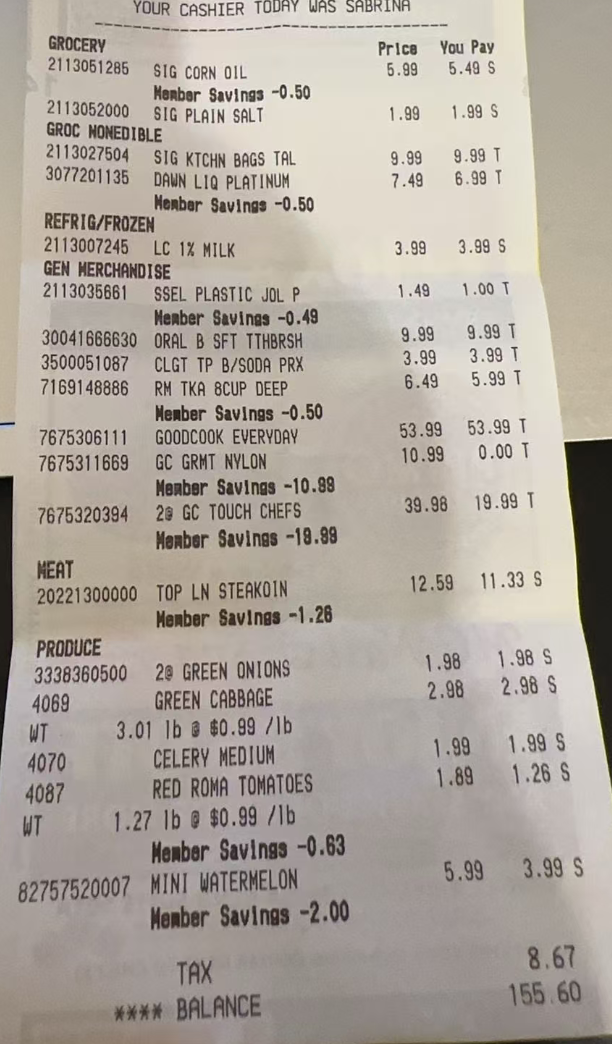
\includegraphics[width=.4\linewidth]{image/交流学习/vons发票.png}
    \caption{Vons商店发票}
\end{figure}


\begin{table}[H]
  \centering
  \caption{购物清单明细}
  \begin{tabular}{|>{\centering\arraybackslash}m{3cm}|>{\arraybackslash}m{5cm}|>{\centering\arraybackslash}m{2cm}|>{\centering\arraybackslash}m{2cm}|}
    \hline
    \textbf{商品类别} & \textbf{商品名称（英文/中文）} & \textbf{原价} & \textbf{实付价} \\
    \hline
    GROCERY（杂货） & SIG corn oil（SIG 玉米油） & 5.99 & 5.49 \\
    \hline
    GROCERY（杂货） & SIG PLAIN SALT（SIG 普通盐） & 1.99 & 1.99 \\
    \hline
    GROCERY（杂货） & SIG KTCHN BAGS TAL（SIG 厨房垃圾袋） & 9.99 & 9.99 \\
    \hline
    GROCERY（杂货） & DAWN LIQ PLATINUM（汰渍白金液体洗洁精） & 7.49 & 6.99 \\
    \hline
    REFRIG/FROZEN（冷藏/冷冻食品） & LC 1\% MILK（LC 1\% 低脂牛奶） & 3.99 & 3.99 \\
    \hline
    GEN MERCHANDISE（一般商品） & SSEL PLASTIC JOL P（塑料容器） & 1.49 & 1.00 \\
    \hline
    ORAL（口腔护理） & ORAL B SFT TTHBRSH（欧乐 B 软毛牙刷） & 9.99 & 9.99 \\
    \hline
    CLGT B FT/BSODA PRX（清洁用品） & CLGT B FT/BSODA PRX & 3.99 & 3.99 \\
    \hline
    RM TKA BCUP DEEP（厨房用品） & RM TKA BCUP DEEP & 6.49 & 5.99 \\
    \hline
    GOODCOOK EVERYDAY（锅） & GOODCOOK EVERYDAY & 53.99 & 53.99 \\
    \hline
    GC GRMT NYLON（砧板；厨房用品） & GC GRMT NYLON & 10.99 & 0.00 \\
    \hline
    2@ GC TOUCH CHEFS（刀） & 2@ GC TOUCH CHEFS（“2@”指2件） & 39.98 & 19.99 \\
    \hline
    MEAT & TOP LN STEAKOIN（顶级牛里脊） & 12.59 & 11.33 \\
    \hline
    PRODUCE & 2@ GREEN ONIONS（2根青葱） & 1.98 & 1.98 \\
    \hline
    PRODUCE & GREEN CABBAGE（绿甘蓝） & 2.98 & 2.98 \\
    \hline
    PRODUCE（ & CELERY MEDIUM（芹菜） & 1.99 & 1.99 \\
    \hline
    PRODUCE & RED ROMA TOMATOES（番茄） & 1.89 & 1.26 \\
    \hline
    PRODUCE & MINI WATERMELON（西瓜） & 5.99 & 3.99 \\
    \hline
  \end{tabular}
  \label{tab:shopping_list}
\end{table}

在美超往往很难买到诸如面条、酱油这样的亚洲食品。线上平台 Weee 上可以买到很多亚洲食材，例如调料（生抽、老抽、酱油等）和方便面（美国本土超市里常见的似乎只有辛拉面）。不过，如果有机会去到亚洲超市，例如 大华（99 Ranch），亚洲食物价格往往便宜。

在美国，公共交通并不发达。如果没有车，通勤就会占据掉大量的时间，生活节奏也会随之慢下来。
但或许，这种慢节奏也是生活的一部分。生活是工作的基础，学会在有限的条件中找到节奏，也正是 trainee 阶段的意义之一。享受烹饪、在厨房里创造美食，本身就是一种治愈。
最后简单总结一下每月的开销：房租1100，电话卡20，公交月卡72，生活费200左右，水电网50。
%20251023-sbp

\subsubsection*{文化与人际}

实习最直接、最现实的收获，无疑是推荐信和论文；但是功利之外，实习更加重要的目的是为了感受未来的工作氛围，为选择做铺垫。作为“申请季逃兵”，我没有申请琐事以及现实的压力，活得自然比同舍生自在得多。

这一次交换让我有了更多的感悟。

首先是氛围不同。国外的实验室国际化程度高，可以接触到不同的思想和文化。

许多华人组文化相近、沟通顺畅，确实更容易融入；但节奏也往往更“紧凑”，少了些多文化交流与英语环境的挑战。我们的实验室PI Xiao是华人，却拥有友善且多元的氛围：成员来自西班牙、墨西哥、台湾、中亚与美国本地，还有一位 UCSD 的华人实习生。刚开始时，面对西班牙师兄的重音一脸懵，也跟不上本地师兄飞快的语速。导师还特意让我跟着去多练听力，多练口语。

其次是他们对于科研以及生活的态度和国内截然不同。

他们的科研与生活态度中都带着一种“松弛感”，这让我这个一生都在追赶 ddl与追求绩点的亚洲学生倍感震撼。  
台湾师兄都40多岁了。曾嫌本土太“卷”，赴日求学，却发现日本的 PI 更倾向“放养”：导师不需要支付学生的学杂费以及工资，导师因此会分配各种看似“不可能”的课题。表面自由，实则艰辛且往往遥遥无期——这或许正是日本科研既高产又高压的写照。  
墨西哥师姐在 Ph.D. committee meeting 上常常“一问三不知”。她来自一个保守的地方，家乡的女性多以贤妻良母为人生信条。她笑着说，16 个女生中，只有 2 个仍在工作——一个是“暂时没找到老公”，另一个就是她。问师姐以后想干什么，她还是一句I don't know.
本地美国师兄毕业于 UCSD，为人随和宽厚，异常勤奋。
那位 UCSD 的华人实习生与我年纪相仿，却令我印象极深：她谦和自信，在不同课题间游刃有余，眼界开阔、行动稳重。她总是说不愿意在高压下工作，但人生总要有一段努力的时光。
还有一位科大强基 21 级的师兄，GPA 4+。和我一样，前路光明我是看不到，道路曲折却又走不完，迷茫于未来要做什么？

我个人认为，重要的一点是国内对于读书的意义的曲解。“读书改变命运”造就了遇事不决就去上学，不管合不合适上学都要挤破头皮争取名额。这种风气之下，内卷越发严重。大学找不到好工作就读研，全军万马过独木桥后又被迫去读博。读博到头又发现也没比本科工资高多少。人的精力有限，皓首穷经近三十载，一无所有不说，还耗尽了探索欲和求知欲。

同样地，国内外关注的重点似乎也不太一样。国内似乎过于看重绩点、排名、publication。

SBP 的 QS 专排只有 100，过去的我或许会对此嗤之以鼻。但这里Ph.D年薪 5 W美元，毕业时长少于5年；每周都有 free food，福利拉满,也许是周围甚至是全美最幸福的研究所之一。当我小心翼翼地问本地师兄“周末要来实验室吗”时，他疑惑地反问周末没实验为什么要来？ 

\begin{figure}[H]
    \centering
    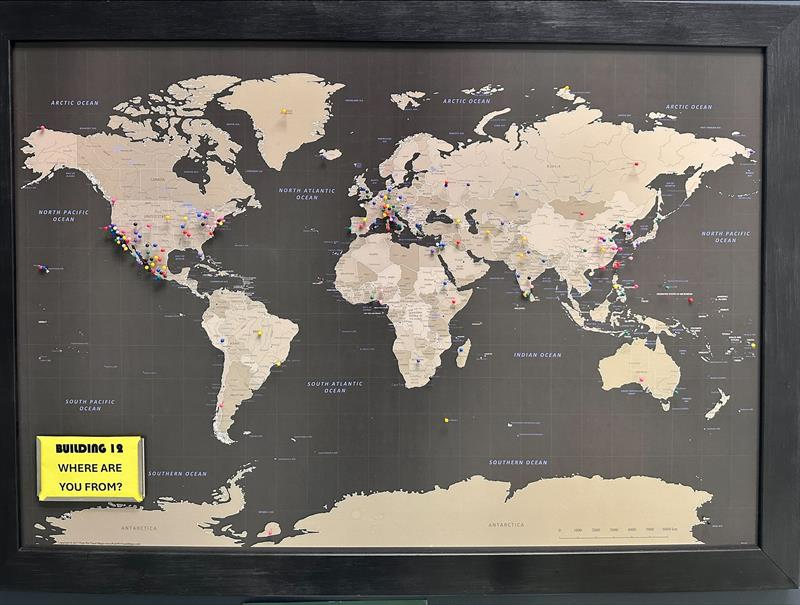
\includegraphics[width=0.6\linewidth]{image/交流学习/where-sbp.jpg}
    \caption{Highly international environment}
\end{figure}

SBP 还常举办各种有趣的活动。比如 10 月 23的 \textit{Postdoc Pitch Competition}，每位博后都有 3 分钟展示自己科研中最“charming”的部分——科研成了脱口秀；欢声笑语中。 
此外，每周的 seminar 对所有人开放，任何人都能无门槛展示自己的 data。科研少不了battle，因为真正的科研都是有limitation的，但是现场没有高高在上的批评与指点，更多的是平等的讨论与灵感的交流。

\begin{minipage}{0.44\textwidth}
  \centering
  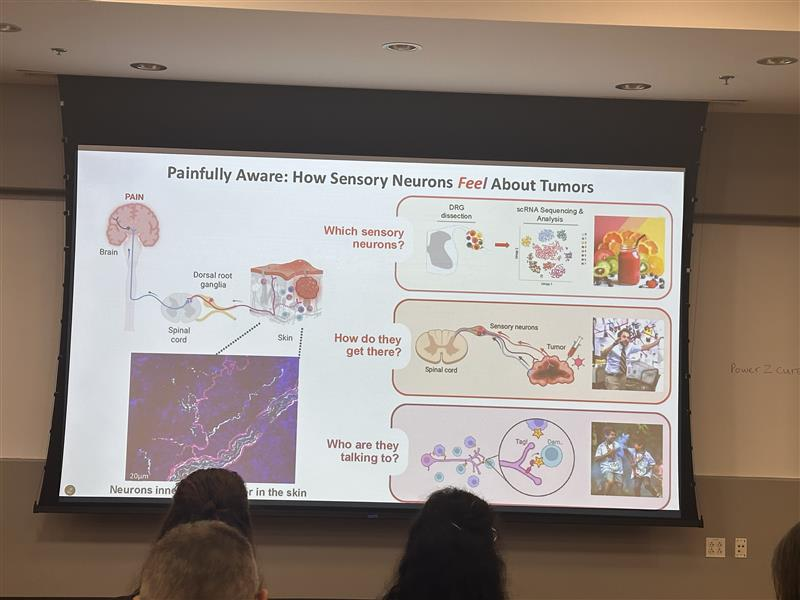
\includegraphics[width=0.9\textwidth]{image/交流学习/sbp-pre1.jpg}
\end{minipage}
\hspace{1em}
\begin{minipage}{0.45\textwidth}
  \centering
  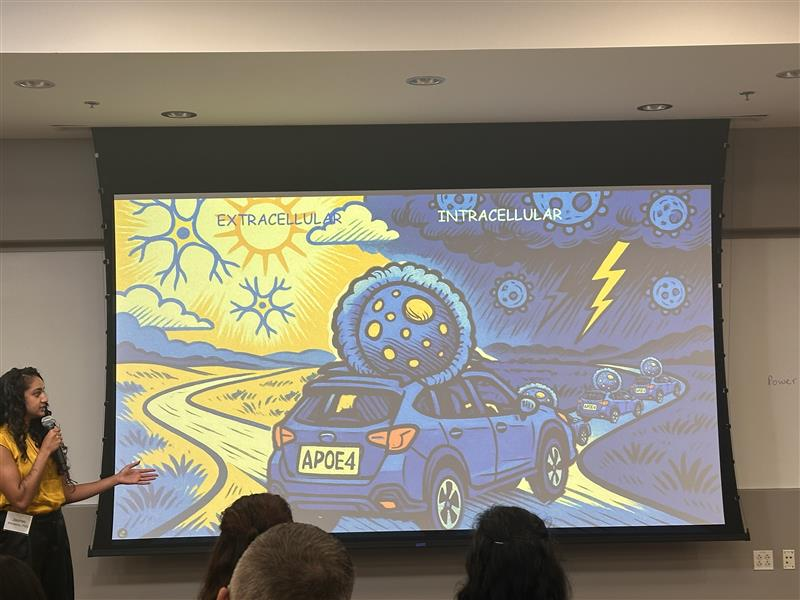
\includegraphics[width=0.9\textwidth]{image/交流学习/sbp-pre2.jpg}
\end{minipage}

这一段经历，让我看到了科研的另一面。也许大家需要冷静地反思一下未来的选择。

%20251024-sbp-待续

还有，我对于美本学生以及国内学生也有了新的认识。
那位美本大三intern的绩点为3.99/4.0，排名40左右；我3.75/4.3，排名10。虽然她认为UCSD让“所有人”绩点都3.99不好，但是在保外以及出国上，实实在在是减分项。更何况国外的committee以及国外的教授，有多少了解国内的高校体制呢？或许在他们眼里，隔壁安徽大学大概是和纽约大学一个层级的吧？

美本的那个intern，她是走国际高中考进UCSD，但是她的大方、高认知、勤奋以及对于知识的渴望让我深感佩服。她是生物信息学，有4篇一作论文，还被编辑邀请参与审稿。让我更确信了一点，优绩主义只能筛选傻子……

以上的部分可以投意林了。下面的部分就要放知乎了。月亮永远是一面亮一面暗。有人的地方就有江湖，美国的人情世故也很严重。我相信大家在师兄师姐口中听过无数次美国connection大于天了吧？另外美国现在很多大学给的津贴低到让人误以为是现实版的“活着”，不少博后挤客厅也不是什么新鲜事。在前面也和大家算过，一个博士（后）的成本5年下来不少于50W，PI 做着做着没钱也是常事。我们PI每天早八晚八，周末加班，一轮轮投funding绝非轻松。
